\documentclass[openright]{report}
\usepackage[utf8]{inputenc}
\usepackage[table]{xcolor}
\usepackage{fancyhdr}
\usepackage{extramarks}
\usepackage{amsmath}
\usepackage{amssymb}
\usepackage{flafter} 
\usepackage{amsthm}
\usepackage{multicol}
\usepackage{amsfonts}
\usepackage{tikz}
\usepackage[plain]{algorithm}
\usepackage{forest}
\usepackage{algpseudocode}
\usepackage{changepage}
\usepackage{siunitx}
\usepackage{wasysym}
\usepackage{mathtools}
\usepackage{titlesec}
\usepackage{indentfirst}
\usepackage{graphicx}
\usepackage{titletoc}
\usepackage{array}
\usepackage[hyphens,spaces,obeyspaces]{url}
\usepackage{tabulary}
\usepackage[labelformat=empty]{caption}
\usepackage[english]{babel}
\usepackage[nottoc]{tocbibind}
\usepackage{chngcntr}
\counterwithout{figure}{chapter}
\usepackage[T1]{fontenc}
\usepackage{listings}
\usepackage{xcolor}
\usepackage[scaled=.85]{beramono}

\newcolumntype{K}[1]{>{\centering\arraybackslash}p{#1}}

\graphicspath{ {images/} }
\usetikzlibrary{automata,positioning}

\usetikzlibrary{shapes.geometric, arrows}

\tikzstyle{startstop} = [rectangle, rounded corners, minimum width=3cm, minimum height=1cm,text centered, draw=black, fill=red!30]
\tikzstyle{io} = [trapezium, trapezium left angle=70, trapezium right angle=110, minimum width=3cm, minimum height=1cm, text centered, draw=black, fill=blue!30]
\tikzstyle{process} = [rectangle, minimum width=3cm, minimum height=1cm, text centered, text width=3cm, draw=black, fill=orange!30]
\tikzstyle{decision} = [diamond, minimum width=3cm, minimum height=1cm, text centered, draw=black, fill=green!30]
\tikzstyle{arrow} = [thick,->,>=stealth]

\renewcommand{\familydefault}{\rmdefault}

\topmargin=-0.45in
\evensidemargin=0in
\oddsidemargin=0in
\textwidth=6.5in
\textheight=9.0in

\linespread{1.25}

\pagestyle{fancy}

\renewcommand{\chaptermark}[1]{\markboth{#1}{}}

\lhead{\projectAuthorShort}
\chead{\reportTopic}
\rhead{\leftmark}
\lfoot{\lastxmark}
\cfoot{\thepage}

\newcommand{\reportTopic}{Phase I and II Report}
\newcommand{\projectAuthorShort}{Cybersecurity Education Group}
\newcommand{\projectTitle}{Hands-on Cybersecurity Education}
\newcommand{\reportDueDate}{February 23, 2018}
\newcommand{\reportClass}{Synthesis Design II}
\newcommand{\reportClassInstructor}{Professor Dana Elzey}
\newcommand{\reportAuthorName}{Clark Benham (cb5ye), Calvin Krist (czk4ja), Saeed Razavi (slr4gf),\\and Jake Smith (jts5np)}
\newcommand{\collaborators}{}

\title{
    \vspace{2in}
    \LARGE{\textbf{\projectTitle}}\\
    \vspace{0.1in}\large{\reportClass:\ \reportTopic}\\
    \vspace{0.1in}\large{\reportClassInstructor}\\
    \normalsize\vspace{0.1in}\large{Due\ on\ \reportDueDate\ at 5:00pm}
    \vspace{1.4in}
}

\author{\reportAuthorName}
\date{}

\renewcommand{\contentsname}{Table of Contents}
\titlespacing*{\chapter}{0pt}{-40pt}{40pt}

\titleformat{\chapter}
  {\Large\bfseries} % format
  {}                % label
  {0pt}             % sep
  {\huge \vspace{-0.2in}}           % before-code

\begin{document}

\maketitle

\large{\tableofcontents}

\chapter{Background}

\section{Introduction}

\par Software is ubiquitous in many countries today. Companies use software to manage user data and offer services. Consumers use it to work, relax, and learn about the world. It's used by governments to help manage elections, recognize citizen needs, and protect their sovereignty. 

\par Software is also used for malicious purposes: criminals, both organized and free-lance, use software, called `malware', to attack businesses, consumers, and governments for personal gain. Malware is also used by activists such as Anonymous to damage those they view as harmful, such as their attack against the World Trade Organization\cite{anonymous_attack}. Even governments use malware for unethical purposes: the NSA's PRSIM program was discovered to be conducting warrantless surveillance on U.S. citizens\cite{nsa_illegal}. High quality programs that costs millions to produce have been used to destroy infrastructure and attack nation states, such as Stuxnet, believed to have been made by the United States\cite{stuxnet}. Autocratic regimes, such as that in Lebanon, use malware to spy on their own people and attack political dissidents\cite{lebanon}.

\par In order to combat malicious software, a specialized security field called `cybersecurity' arose that protects software systems and responds to attacks through a variety of means. Cybersecurity professionals from Gartner, an IT research company, defined the term as "security practices related to the combination of offensive and defensive actions involving or relying upon information technology and/or operational technology environments and systems"\cite{cyber_def}. In other words, the field of cybersecurity encompasses both attacking and defending systems such as computers, networks, and databases. Due to the components of these systems, cybersecurity professionals are often also called IT security professionals. This field is taught at many Universities today, and cybersecurity professionals are in high demand from both companies and governments due to the extreme integration of software into modern society and the high value of user data.

\section{Market Need}

\par At the most superficial level, malware hurts the economy and people's lives. Cyber attacks cost the global economy \$400 billion annually, and is only increasing. This cost largely comes from stealing user data, such as credit cards and medial information, and by shutting down company infrastructure. There are thousands of such attacks world-wide: in 2016, there was over 1000 data breaches of U.S. companies alone. For example, Maersk, the shipping company, had all their computer systems infected by ransomware (malware that stops the user from doing anything until they pay a fee). This completely halted their operations for over a week as they switched back to pen-and-paper management and quickly rebuilt all their servers and databases from the ground up. This attack, which did not even target the company, cost them about \$250 million\cite{maersk}. Another example comes from 2017, when Equifax was hacked, exposing the personal data of over 160 million Americans - data that included credit card numbers, social security numbers, and more. This allows criminals to steal people's identity and conduct all types of fraud.

\par It should be noted that it's not always the economy or individuals who are hurt: political systems and entire cultures can be damaged as well. For example, Russia's hacking of the elections compromised the integrity and sovereignty of the United States\cite{russa_indicement}. The operations consisted largely of leaking DNC emails and an extensive online disinformation campaign on social media, disguising the foreign influence through special servers and long-term user accounts\cite{russa_indicement_nyt}\cite{what_russia_did}. This is a corruption of the democratic culture, and could have long term effects both nationally and internationally. 

\par Autocratic regimes, or even those with a less democratic culture than the United States, often use surveillance software (spyware) to spy on political dissidents and journalists trying to report on 'politically harmful' information. As a result, many companies sell 'security solutions' to autocratic regimes such as Ethiopia which are used to spy on their citizens\cite{ethiopia_surveillance}. Mobile devices can be turned into tools of repression, where messages one sends to others expressing dissatisfaction can be means for arrest or other forms of retaliation. Countries like Saudi Arabia own large shares in infamous cyber security companies and use their products for espionage on their own \cite{saudi_cyber}. Mexico illegally uses hacking tools to spy on activists and reporters in order to intimidate and harass them\cite{mexico_cyber}. In other words, malware is actively used to support autocratic and politically harmful practices.

\par Part of this excess of cyber attacks and malware comes from the fact that IT security professionals have to defend entire systems that have hundreds of vulnerabilities, while attackers have to find just one weak point. In other words, attacking is inherently easier than defending. However, there also aren't enough qualified cybersecurity professionals for all the businesses and governments in any country, leaving user data vulnerable to attack. 90\% of companies worldwide say they are unprepared for cyber attacks, and governments similarly have trouble. 70\% of U.S. federal IT security professionals say the government lacks qualified employees, and 86\% say they have trouble finding personal to fill spots\cite{fed_cs_jobs}. It is estimated that, by 2020, there will be 1.5 million unfilled cybersecurity jobs in the U.S., leaving the way open for user data and companies to be more vulnerable than ever\cite{why_no_cyber_classes}.

\par The direct cause of this issue can be seen in a report made by the ISACA in 2017, an international association of IT professionals. They surveyed members of their association and found that most IT security job posting just get around 5 responses, and only around 10\% of job postings get at least 20 responses. In contrast, most corporate job openings receive between 60 and 250 applicants\cite{job_survey}. This is because \textit{everyone} needs IT security professionals, and there are not enough of them to go around.

\par This problem is further compounded by the fact that few of those who even respond to cybersecurity job postings are qualified: the ISACA found in their survey that nearly half of those questioned said that one in four of respondents to their job posting are qualified. The number one reason potential hires were unqualified was a lack of hands one experience\cite{job_survey}. In other words, not only do very few people respond: an astounding proportion of respondents are un-hireable. This leaves the whole world without the necessary number of cybersecurity experts to protect them.

\section{Observations}

\section{Problem Identification}

\par Why are there so few cybersecurity job applicants and why are so few of them qualified? To begin, this is a very new field. As a result, there is no consensus as to what students should be taught and how they should be taught\cite{why_no_cyber_classes}. This means that there can be a large discrepancy between what employers want, what employers need, and what students are taught. Furthermore, not many universities offer undergraduate degrees in cybersecurity, much less a quality education in the field. This includes the University of Virginia. Here at UVA, there is currently a lot of debate between CS professors as to how much security education should be required to get a degree. Currently, while numerous security courses are offered and more are coming, there is no requirement to take one\cite{comsci_handbook}. Students only study cybersecurity if it interests them. This is not uncommon in United States universities.

\par This results in two things: normal software developers leave more vulnerabilities in their applications, and less students become interested in cybersecurity. Not teaching basic security to CS undergraduates means that those students, now professional developers, are not aware of the security needs of applications or the ways that they can expose user data. This means lots of software, much of which is used by consumers, have vulnerabilities that can be abused by malicious hackers. If graduates were required to take basic security courses, they may be more cognizant of the security of their applications and consumers would be safer.

\par Furthermore, because many universities do not require that students take security courses, many students do not. Cybersecurity, in contrast to most of computer science, is very intimidating. It has a dry reputation, and it's generous to say that there even \textit{basics} to cybersecurity. As we have seen by talking with students, many don't know where to begin studying the topic. 

\par Cybersecurity requires vast domain experience due to the diversity of systems that need to be protected. As a result, it's hard to learn and hard to become passionate about because there is no immediate payoff to studying it. This means that few students will become interested in the field on their own, and without universities pushing students towards towards the field, this problem will not be rectified.

\par Even for those who decide cybersecurity is a topic worth pursuing, there are many barriers. Much of cybersecurity is about the interaction of systems. This means that to do more than read about topics--to get hands on experience--students need to be able to set up or simulate the systems they read about. Students need to know more than just intermediate programming and network theory: they also need to be server experts, OS experts, and knowledgeable about service architecture. 

\par This asks a lot of students. The necessary complexity of these systems makes them difficult to set up, and even following an online tutorial is frustrating. Small differences in computer configurations can result in hours of hard work debugging the problem. This is very discouraging, and can slow down student learning or even dissuade them from the field entirely. 

\par These same problems are why many university graduates lack hands on experience and are unqualified for most IT security jobs. Because of the nature of teaching in a classroom, the labs have to work for all students. If the lab doesn't work on one student's computer, the professor is faced with a painful decision: to leave the student behind, or hold up the whole class to try and debug the issue. As a result, most labs are as simple as possible while still demonstrating core concepts to reduce the time spent setting up and the risk of a student not being able to participate\cite{ibrahiminterview}. This means that, for universities to give students hands on experience, the best technology right now is to have dedicated computer labs set up for students to use. A computer for every student, enough routers and servers for all of them, the databases necessary. This would be incredibly expensive, take lots of time to set up, test, and prepare, and it still could fail.

\par The result is that schools can't give students hands on experience and students have lots of trouble getting that experience themselves. Thus, most of those that do choose to study this field lack the requisite experience necessary to be a qualified IT security professional.

\begin{center}
    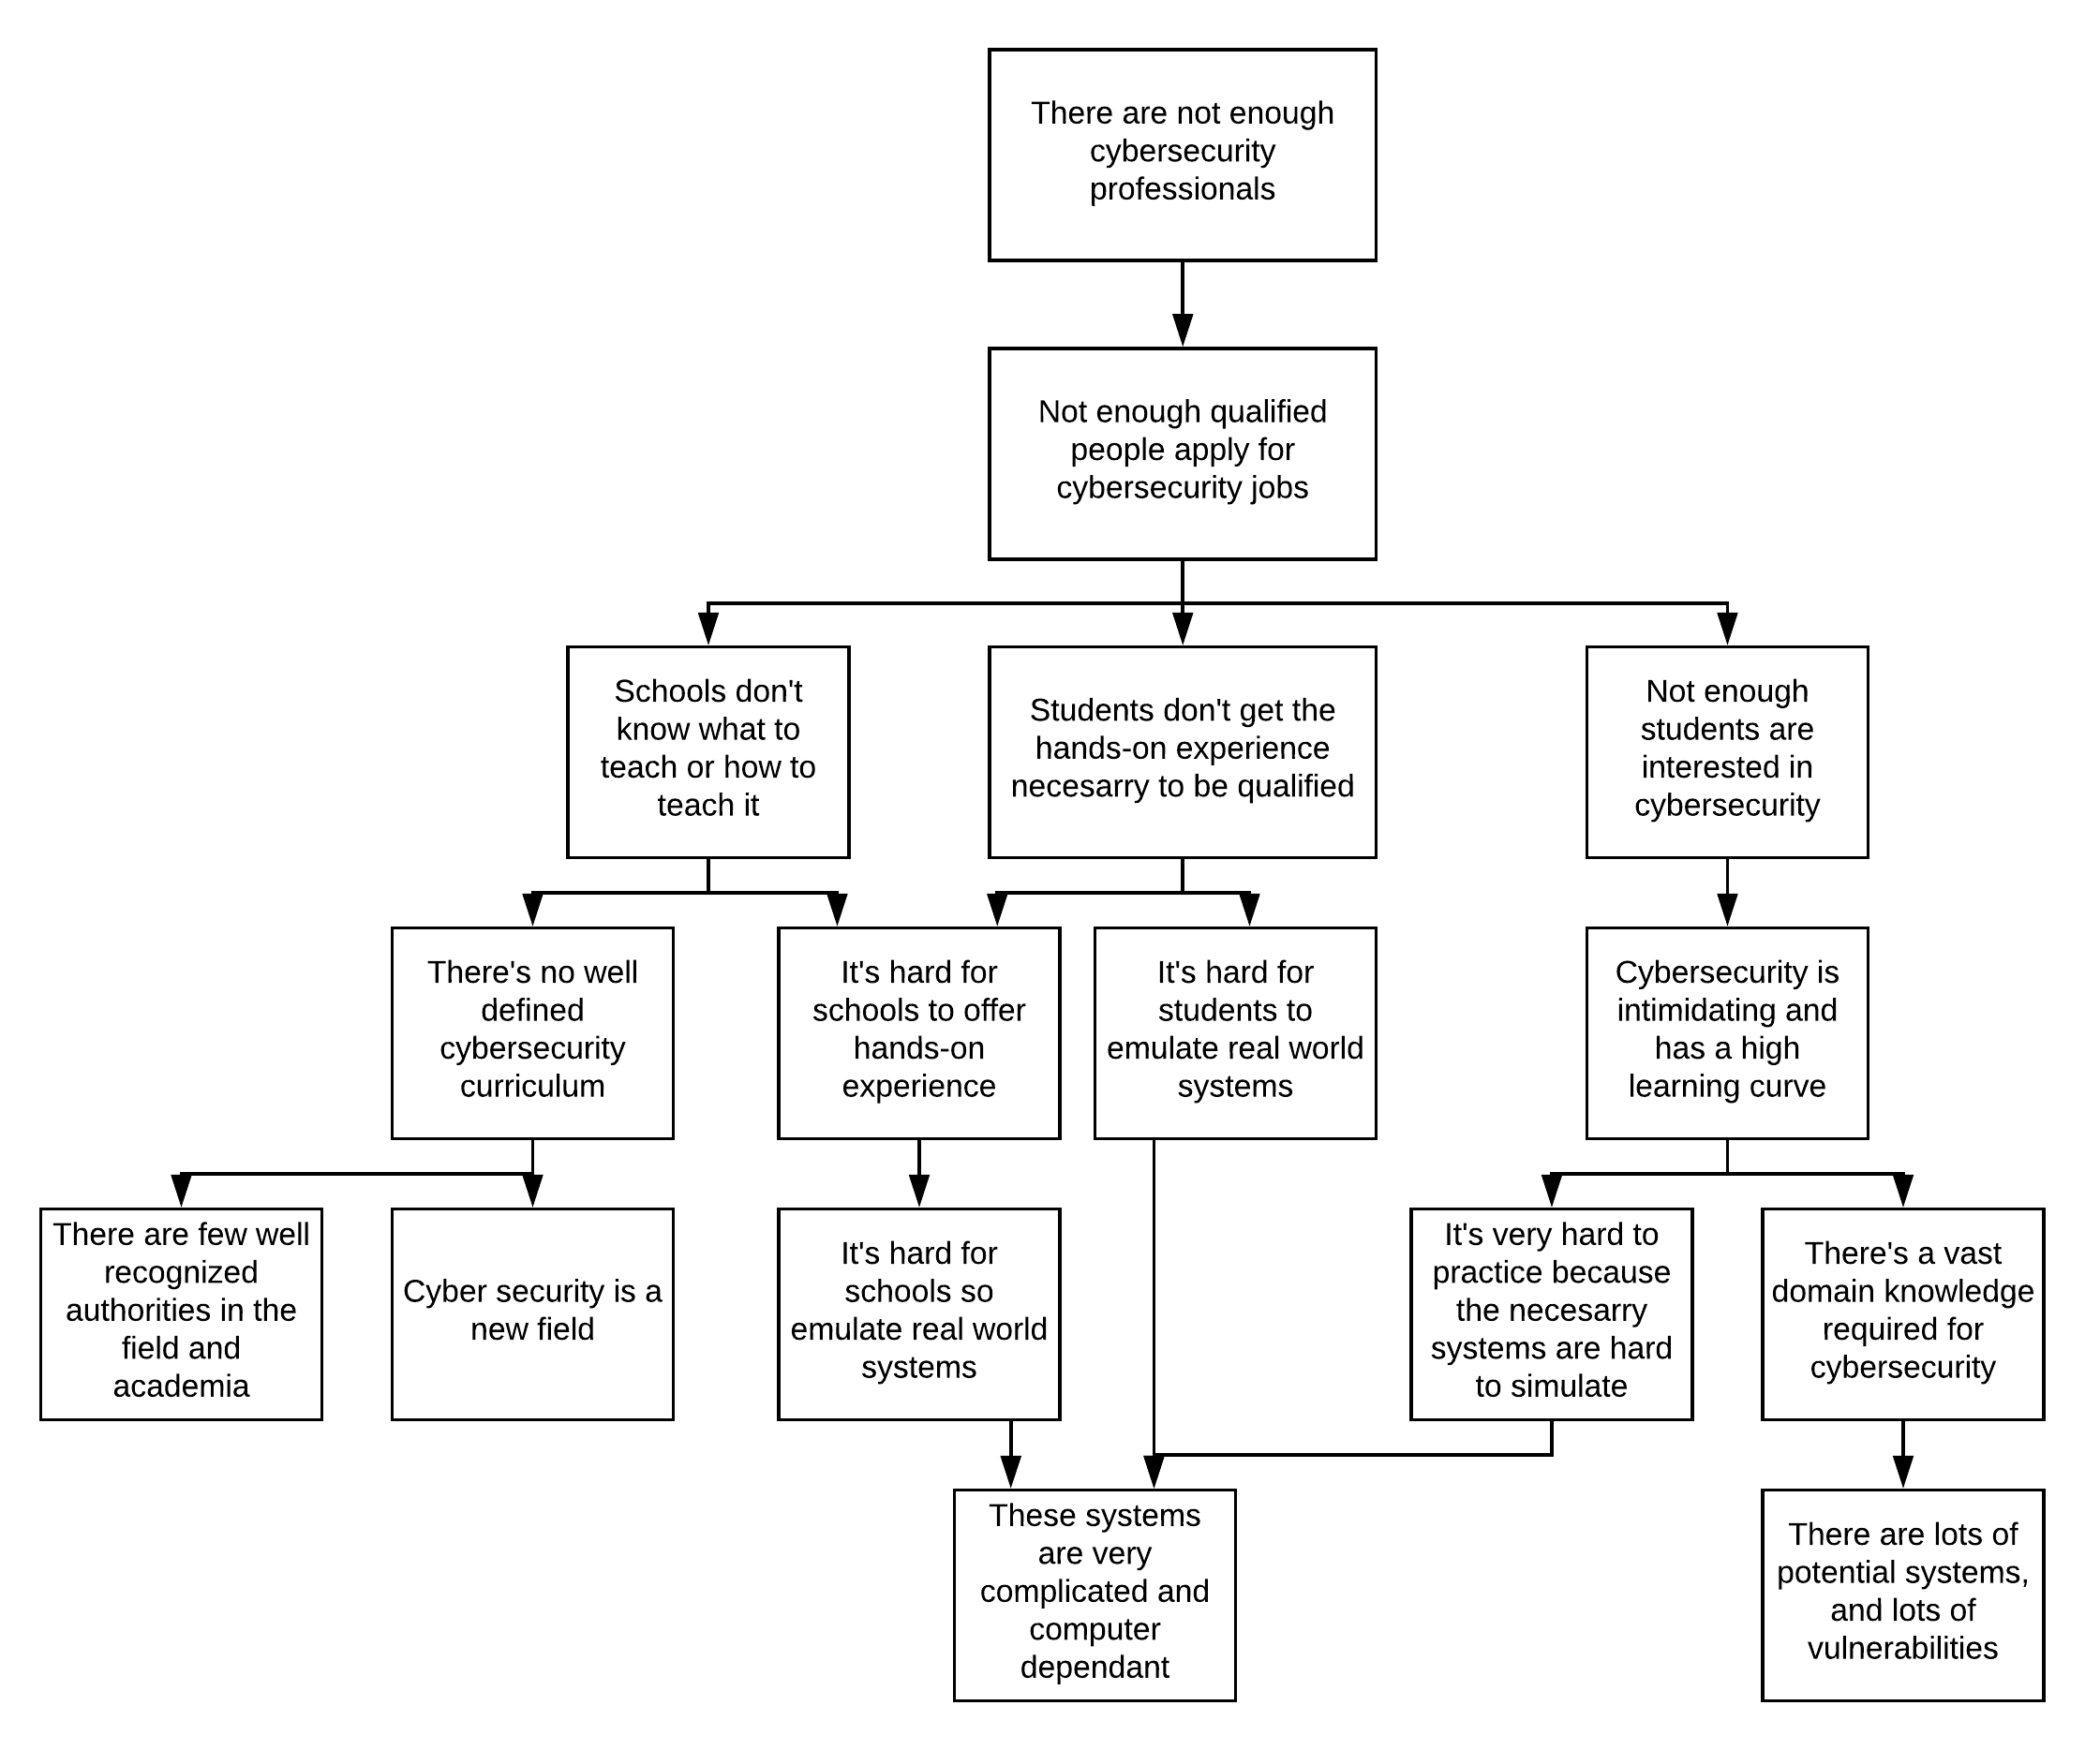
\includegraphics[scale=0.34]{images/Why-Why.png}
    \captionof{figure}{\textbf{Figure \arabic{figure}:} Why-Why Diagram identifying the problem}
\end{center}

\par As can be seen in Figure 1, there are a few different conclusions that can be drawn. As has been discussed, cybersecurity is complicated because the systems it needs to defend are complicated: that can't be changes. However, the other two main lines of inquiry that the diagram shows--hands-on experience is hard to achieve due to the complexity of the systems, and there is no well defined curriculum--can both be targeted.

\section{Prior Art}

\par one thing to mention here that we didn't in our presentation is how many governments are pouring MILLIONS into cyber programs. that is, technically, prior art.

\par see "The \$19 billion cybersecurity initiative President Obama proposed earlier this year included \$62 million for a new CyberCorps Reserve program that would train and provide scholarships to people who take cybersecurity jobs with the federal government" from \cite{why_no_cyber_classes}


\section{Resources}

\chapter{Solution Identification}

\section{Context}
****************JAKE****************
-economic: students / beginners do not want to pay for products until they prove to be useful, subscription models are more popular for learning content, lots of potentially competing similar free infosec training resources, trend towards open-source projects

socio-cultural: target age remains constant - generations of new students in high school/college looking to learn cybersecurity, also adults looking to learn/practice cybersecurity, cybersecurity is a fast growing industry - field is in high demand of quality solutions, trend towards people deciding to study 

-how do the problem and potential solutions interact with the socio-cultural, organizational, economic, political,…context? 

\section{Customers and Stakeholders}
****************JAKE****************
-CCDC Team
-GE
-UVA Infosec Professors

\section{Constraints}
****************JAKE****************
TALK ABOUT MITIGATIONS

\subsection{Project Risks}
**************** JAKE ****************
-Software performance and capabilities
-Complicated tech stack configuration

\subsection{Project Resources}
****************JAKE****************
-Limited hardware for testing
-Distribution of cybersecurity knowledge

\subsection{Project Costs}
****************JAKE****************
-All software and tools are free
-Potentially upgrade development hardware

\subsection{Project Quality}
****************JAKE****************
-Easy for instructor
-Easy for student
-Easy for professional
-Helpful for all
-MORE ON PROJECT part

\subsection{Product Scope}
****************JAKE****************
-Free
-Machine and subject material apathetic
-Easy setup, low required tech specs
-Models complex, realistic machine configurations
-Limits user ability at and desire for unethical hacking or damage of P.M.

\section{Brainstorming}

\par 

\section{Solution Identification}

\section{Approach}
****************JAKE****************
c and p some stuff from our scrum proposal

\par more example text\cite{ibrahiminterview}. Example graphic

\begin{center}
    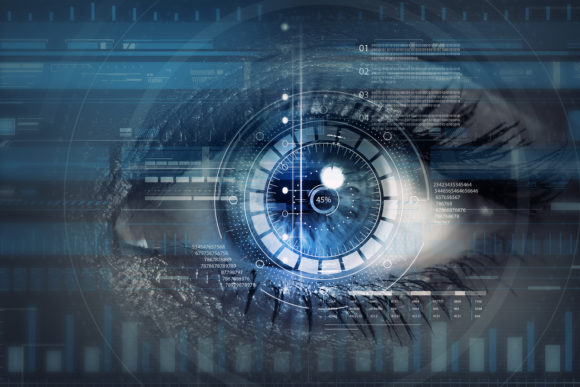
\includegraphics[scale=1]{images/cyber.jpg}
    \captionof{figure}{\textbf{Figure \arabic{figure}:} Example figure caption}
\end{center}

%Sets the bibliography style to UNSRT and imports the 
%bibliography file "samples.bib".

\bibliographystyle{unsrt}
\bibliography{Bibliographies/Phase_I_II.bib}


\listoffigures
\cleardoublepage


\end{document} 